\documentclass[10pt]{article}
\usepackage[utf8]{inputenc}
\usepackage{amsmath}
\usepackage{amssymb}
\usepackage{graphicx}
\usepackage{geometry}
\usepackage{enumitem}
\usepackage{multicol}
\usepackage{tabularx}
\usepackage[table,xcdraw]{xcolor}
\usepackage{array}
\usepackage{ifthen}
\usepackage{tikz}
\usetikzlibrary{shapes,arrows,positioning,calc}

\geometry{a4paper, margin=1in}
\pagestyle{empty}

\newboolean{showresults}
\setboolean{showresults}{false} % Set to true to show solutions

\begin{document}

% COVER PAGE
\begin{center}
\vspace*{2cm}
{\Huge\textbf{University of Nebraska-Lincoln}}\\[1cm]
{\LARGE\textbf{ECEN 463/863 - Digital Signal Processing}}\\[0.5cm]
{\Large\textbf{Midterm Exam}}\\[2cm]

{\large\textbf{October 29, 2025}}\\[3cm]

\begin{tabular}{|c|c|c|}
\hline
\textbf{Question} & \textbf{Points} & \textbf{Score} \\
\hline
1 & 20 & \hspace{2cm} \\
\hline
2 & 20 & \hspace{2cm} \\
\hline
3 & 20 & \hspace{2cm} \\
\hline
4 & 20 & \hspace{2cm} \\
\hline
5 & 20 & \hspace{2cm} \\
\hline
\textbf{Total} & \textbf{100} & \hspace{2cm} \\
\hline
\end{tabular}

\vspace{3cm}

\noindent\textbf{Name:} \underline{\hspace{8cm}}\\[1cm]

\vspace{2cm}

\begin{center}
\textit{"On my honor, I have neither given nor received aid on this exam"}
\end{center}

\vspace{1cm}



\noindent\textbf{Student Signature:} \underline{\hspace{8cm}}\\[0.5cm]

\end{center}

\newpage

% -------------------------------------------- QUESTION 1 PAGE --------------------------------------------

\begin{enumerate}
    \item \textbf{(20 points)} For each of the following input/output relations for a discrete time system, please indicate whether the system is:

\begin{itemize}[left=0pt, labelwidth=*, align=left]
    \item[\bf{L} or \bf{NL}:] Linear or Not Linear
    \item[\bf{TI} or \bf{NTI}:] Time Invariant or Not Time Invariant
    \item[\bf{C} or \bf{NC}:] Causal or Not Causal
    \item[\bf{B} or \bf{NB}:] BIBO Stable or Not BIBO Stable
\end{itemize}

\noindent 
If for any property it is not possible to say, then indicate this by writing \textbf{CBD} (Cannot Be Determined).

\vspace{0.5cm}

\ifthenelse{\not{\boolean{showresults}}}{
\renewcommand{\arraystretch}{1.5}
\begin{table}[h!]
\centering
\begin{tabularx}{\textwidth}{|>{\raggedright\arraybackslash}X|c|c|c|c|}
    \hline
    \textbf{Input/Output Relation} & \textbf{L/NL} & \textbf{TI/NTI} & \textbf{C/NC} & \textbf{B/NB} \\
    \hline
    $y[n] = 3x[n-1] + 2x[n-3] - x[n-7]$ & & & & \\
    \hline
    $y[n] = x[n] \cdot x[n-2] + 5$ & & & & \\
    \hline
    $y[n] = \sum_{k=0}^{3} x[n-k] \left(\frac{1}{2}\right)^k$ & & & & \\
    \hline
    $y[n] = x[2n] + \sin(0.1\pi n)$ & & & & \\
    \hline
    $y[n] = \max\{x[n], x[n-1], x[n-4]\}$ & & & & \\
    \hline
\end{tabularx}
\end{table}
}{}


\noindent \textbf{Notes:}
\begin{enumerate}[left=0pt, labelwidth=*, align=left]
    \item In our notation, if the upper limit of a summation is higher than or equal to the lower limit, a summation occurs; otherwise, the summation returns a zero.
    \item $\operatorname{max}\{\}$ returns the maximum of three values -- e.g., $\operatorname{max}\{7, -3, 10\} = 10$.
    \item Show all work you did to obtain your answers. You can either show that the relation meets our definition, or show a counter-example that shows the relation does not. 
\end{enumerate}


\ifthenelse{\boolean{showresults}}{
\renewcommand{\arraystretch}{1.5}
\begin{table}[h!]
\centering
\begin{tabularx}{\textwidth}{|>{\raggedright\arraybackslash}X|c|c|c|c|}
    \hline
    \textbf{Input/Output Relation} & \textbf{L/NL} & \textbf{TI/NTI} & \textbf{C/NC} & \textbf{B/NB} \\
    \hline
    $y[n] = 3x[n-1] + 2x[n-3] - x[n-7]$ 
    & L    % Linear combination of delayed inputs
    & TI   % Delays are constant
    & C    % Only depends on past inputs
    & B    % Bounded input gives bounded output
    \\
    \hline
    $y[n] = x[n] \cdot x[n-2] + 5$ 
    & NL   % Multiplication of inputs is nonlinear
    & TI   % Time delays are constant
    & C    % Only depends on present and past
    & NB   % Product can be unbounded even if inputs are bounded
    \\
    \hline
    $y[n] = \sum_{k=0}^{3} x[n-k] \left(\frac{1}{2}\right)^k$ 
    & L    % Linear combination (FIR filter)
    & TI   % Coefficients and delays are constant
    & C    % Only past and present inputs
    & B    % Sum of exponentially weighted terms is bounded
    \\
    \hline
    $y[n] = x[2n] + \sin(0.1\pi n)$ 
    & NL   % Downsampling (x[2n]) plus additive term
    & NTI  % sin(0.1πn) makes it time-varying
    & C    % Only depends on current time sample
    & B    % Bounded if x[n] is bounded (sine is always bounded)
    \\
    \hline
    $y[n] = \max\{x[n], x[n-1], x[n-4]\}$ 
    & NL   % Max operation is nonlinear
    & TI   % Delays are constant
    & C    % Only present and past inputs
    & B    % Max of bounded inputs is bounded
    \\
    \hline
\end{tabularx}
\end{table}

\vspace{0.5cm}

\textbf{Solution Explanations:}

\textbf{System 1:} $y[n] = 3x[n-1] + 2x[n-3] - x[n-7]$
\begin{itemize}
    \item \textbf{Linear:} Satisfies superposition principle - linear combination of delayed inputs
    \item \textbf{Time-Invariant:} Delays are constant, no explicit dependence on n
    \item \textbf{Causal:} Output only depends on present and past inputs (n-1, n-3, n-7)
    \item \textbf{BIBO Stable:} If $|x[n]| \leq M$, then $|y[n]| \leq (3+2+1)M = 6M$
\end{itemize}

\textbf{System 2:} $y[n] = x[n] \cdot x[n-2] + 5$
\begin{itemize}
    \item \textbf{Nonlinear:} Multiplication of inputs violates superposition
    \item \textbf{Time-Invariant:} No explicit time dependence
    \item \textbf{Causal:} Only uses present and past inputs
    \item \textbf{Not BIBO Stable:} Even if $|x[n]| \leq M$, $|y[n]|$ can be as large as $M^2 + 5$
\end{itemize}

\textbf{System 3:} $y[n] = \sum_{k=0}^{3} x[n-k] \left(\frac{1}{2}\right)^k$
\begin{itemize}
    \item \textbf{Linear:} Weighted sum of delayed inputs (FIR filter)
    \item \textbf{Time-Invariant:} Coefficients and delays are constant
    \item \textbf{Causal:} Only present and past inputs (n, n-1, n-2, n-3)
    \item \textbf{BIBO Stable:} $|y[n]| \leq M(1 + \frac{1}{2} + \frac{1}{4} + \frac{1}{8}) = \frac{15M}{8}$
\end{itemize}

\textbf{System 4:} $y[n] = x[2n] + \sin(0.1\pi n)$
\begin{itemize}
    \item \textbf{Nonlinear:} Downsampling operation x[2n] is nonlinear
    \item \textbf{Not Time-Invariant:} $\sin(0.1\pi n)$ term varies with time
    \item \textbf{Causal:} Only depends on input at current (scaled) time
    \item \textbf{BIBO Stable:} $|y[n]| \leq |x[2n]| + 1 \leq M + 1$ if $|x[n]| \leq M$
\end{itemize}

\textbf{System 5:} $y[n] = \max\{x[n], x[n-1], x[n-4]\}$
\begin{itemize}
    \item \textbf{Nonlinear:} Max operation doesn't satisfy superposition
    \item \textbf{Time-Invariant:} Delays are constant
    \item \textbf{Causal:} Only present and past inputs
    \item \textbf{BIBO Stable:} Max of bounded inputs is bounded: $|y[n]| \leq M$
\end{itemize}

}{}



% \noindent \textbf{Notes:}
% \begin{enumerate}[left=0pt, labelwidth=*, align=left]
%     \item Show your work clearly for each classification.
%     \item For linearity, consider the superposition principle: $T\{ax_1[n] + bx_2[n]\} = aT\{x_1[n]\} + bT\{x_2[n]\}$
%     \item For time-invariance, check if $T\{x[n-n_0]\} = y[n-n_0]$ for any delay $n_0$
%     \item For causality, ensure output depends only on present and past inputs
%     \item For BIBO stability, show that bounded input produces bounded output
% \end{enumerate}




% -------------------------------------------- QUESTION 2 PAGE --------------------------------------------
\newpage

\item \textbf{(20 points)} For each of the following sequences, please indicate "yes" it is an eigensequence or "no" it is not an eigensequence for discrete-time LTI systems.

\vspace{0.5cm}

\begin{enumerate}[label=(\alph*)]
    \item $x_1[n] = \left(\frac{1}{3}\right)^n u[n]$ 
    
    \vspace{3cm}

    \item $x_2[n] = e^{j\frac{2\pi}{3} n}$

    \vspace{3cm}
    
    \item $x_3[n] = \cos(\frac{\pi}{5} n)$
    
    \vspace{3cm}
    
    \item $x_4[n] = \delta[n-3]$ 
    
    \vspace{3cm}

    \item $x_5[n] = 3$ 
    
    \vspace{3cm}
\end{enumerate}

\ifthenelse{\boolean{showresults}}{
\vspace{0.5cm}
\textbf{Solutions:}

\begin{enumerate}[label=(\alph*)]
    \item $x_1[n] = \left(\frac{1}{3}\right)^n u[n]$ \hfill Answer: \textbf{Yes}
    
    This is a causal exponential sequence of the form $z^n u[n]$ where $z = \frac{1}{3}$. For any LTI system with impulse response $h[n]$, the output is $y[n] = H(z) \cdot z^n u[n]$ where $H(z)$ is the transfer function evaluated at $z = \frac{1}{3}$. Since $|z| = \frac{1}{3} < 1$, this converges for stable systems.
    
    \vspace{0.5cm}
    
    \item $x_2[n] = e^{j0.4\pi n}$ \hfill Answer: \textbf{Yes}
    
    This is a complex exponential of the form $e^{j\omega_0 n}$ where $\omega_0 = 0.4\pi$. Complex exponentials are eigensequences of LTI systems with eigenvalue $H(e^{j\omega_0})$, where $H(e^{j\omega})$ is the frequency response evaluated at $\omega = 0.4\pi$.
    
    \vspace{0.5cm}
    
    \item $x_3[n] = \cos(0.2\pi n + \frac{\pi}{4})$ \hfill Answer: \textbf{No}
    
    While sinusoidal sequences can be eigensequences, this cosine with a phase shift is not a pure eigensequence. It can be written as a linear combination of complex exponentials: $\cos(0.2\pi n + \frac{\pi}{4}) = \frac{1}{2}[e^{j(0.2\pi n + \pi/4)} + e^{-j(0.2\pi n + \pi/4)}]$, but the individual sequence itself is not an eigensequence.
    
    \vspace{0.5cm}
    
    \item $x_4[n] = 2^n u[-n-1]$ \hfill Answer: \textbf{Yes}
    
    This is an anti-causal exponential sequence. It can be written as $x_4[n] = (2)^n u[-n-1]$, which is of the form $z^n$ for the anti-causal region where $z = 2$. For LTI systems, this is an eigensequence with eigenvalue $H(z)$ evaluated at $z = 2$, provided the ROC of the system includes $|z| = 2$.
    
    \vspace{0.5cm}
    
    \item $x_5[n] = \delta[n-3]$ \hfill Answer: \textbf{No}
    
    The unit impulse function (delayed or not) is not an eigensequence. When $\delta[n-3]$ is input to an LTI system with impulse response $h[n]$, the output is $h[n-3]$ (the impulse response delayed by 3 samples), which is not a scalar multiple of the input unless $h[n]$ has a very specific form.
    
\end{enumerate}

}{}
\vspace{0.5cm}
\textbf{Note:} 
\begin{itemize}
    \item $u[n]$ denotes unit step function
    \item $\delta[n]$ denotes unit impulse (delta) function
\end{itemize}





% -------------------------------------------- QUESTION 3 PAGE --------------------------------------------
\newpage

\item \textbf{(20 points)} Consider the system in the figure below (where $|a| < 1$):
\begin{center}
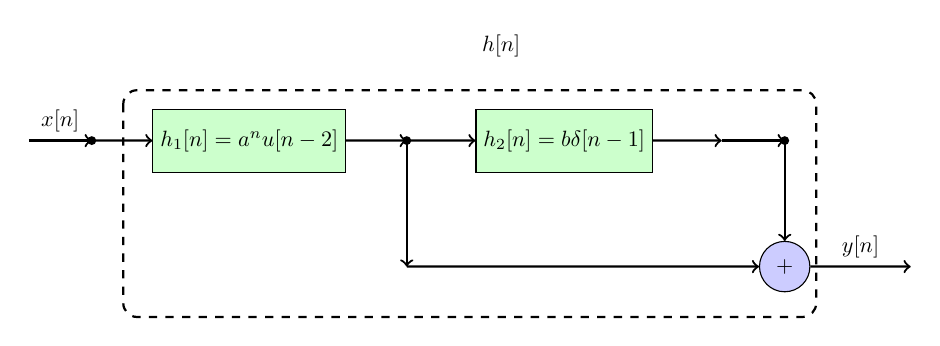
\begin{tikzpicture}[scale=0.8, every node/.style={scale=0.8}]
    % Define styles
    \tikzset{
        block/.style={draw, rectangle, minimum height=1cm, minimum width=2.5cm, fill=green!20},
        sum/.style={draw, circle, minimum size=8mm, fill=blue!20},
        arrow/.style={->, thick},
        system/.style={draw, dashed, thick, rounded corners=5pt}
    }
    
    % Place nodes
    \node[coordinate] (input) at (0,1) {};
    \node[coordinate] (branch1) at (1,1) {};
    \node[block] (h1) at (3.5,1) {$h_1[n] = a^nu[n-2]$};
    \node[coordinate] (a_out) at (6,1) {};
    \node[coordinate] (branch_a) at (6,1) {};
    \node[block] (h2) at (8.5,1) {$h_2[n] = b\delta[n-1]$};
    \node[coordinate] (b_out) at (11,1) {};
    \node[coordinate] (a_down) at (6,-1) {};
    \node[coordinate] (b_right) at (12,1) {};
    \node[sum] (sum_final) at (12,-1) {$+$};
    \node[coordinate] (output) at (14,-1) {};
    
    % Draw the system boundary (dotted box around entire system)
    \draw[system] (1.5,1.8) rectangle (12.5,-1.8);
    
    % Draw arrows
    \draw[arrow] (input) -- node[above] {$x[n]$} (branch1);
    \draw[arrow] (branch1) -- (h1);
    \draw[arrow] (h1) -- (branch_a);
    \draw[arrow] (branch_a) -- (h2);
    \draw[arrow] (h2) -- (b_out);
    \draw[arrow] (branch_a) -- (a_down);
    \draw[arrow] (a_down) -- (sum_final);
    % b[n] arrow going right then vertically down to summation circle
    \draw[arrow] (b_out) -- (b_right);
    \draw[arrow] (b_right) -- (sum_final.north);
    \draw[arrow] (sum_final) -- node[above] {$y[n]$} (output);
    
    % Mark branch points
    \fill (branch1) circle (2pt);
    \fill (branch_a) circle (2pt);
    \fill (b_right) circle (2pt);
    
    % Label overall system
    \node[above] at (7.5,2.2) {$h[n]$};
\end{tikzpicture}
\end{center}

\begin{enumerate}[label=(\alph*)]
    \item \textbf{(8 points)} Find the impulse response $h[n]$ of the overall system.
    
    \vspace{6cm}
    
    \item \textbf{(8 points)} Find the frequency response $H(e^{j\omega})$ of the overall system.
    
    \vspace{6cm}
    
    \item \textbf{(4 points)} Specify a difference equation that relates the output $y[n]$ to the input $x[n]$.
    
    \vspace{4cm}
\end{enumerate}

\ifthenelse{\boolean{showresults}}{
\vspace{0.5cm}
\textbf{Solutions:}

\begin{enumerate}[label=(\alph*)]
    \item \textbf{Finding the impulse response $h[n]$:}
    
    From the block diagram, let's define the intermediate signals:
    \begin{align}
    w[n] &= x[n] * h_1[n] = x[n] * a^nu[n-2]\\
    z[n] &= w[n] * h_2[n] = w[n] * b\delta[n-1] = bw[n-1]
    \end{align}
    
    The overall output is:
    \begin{align}
    y[n] &= w[n] + z[n] = w[n] + bw[n-1]
    \end{align}
    
    For the impulse response, let $x[n] = \delta[n]$:
    \begin{align}
    w[n] &= \delta[n] * a^nu[n-2] = a^nu[n-2]\\
    z[n] &= bw[n-1] = ba^{n-1}u[n-3]
    \end{align}
    
    Therefore:
    \begin{align}
    h[n] &= w[n] + z[n]\\
    &= a^nu[n-2] + ba^{n-1}u[n-3]
    \end{align}
    
    \[
    \boxed{h[n] = \begin{cases}
    0 & \text{if } n < 2\\
    a^n & \text{if } n = 2\\
    a^n + ba^{n-1} & \text{if } n \geq 3
    \end{cases}}
    \]
    
    \vspace{0.5cm}
    
    \item \textbf{Finding the frequency response $H(e^{j\omega})$:}
    
    Taking the DTFT of each subsystem:
    \begin{align}
    H_1(e^{j\omega}) &= \sum_{n=2}^{\infty} a^n e^{-j\omega n} = e^{-j2\omega} \sum_{n=2}^{\infty} (ae^{-j\omega})^n\\
    &= e^{-j2\omega} \cdot \frac{a^2}{1-ae^{-j\omega}} = \frac{a^2 e^{-j2\omega}}{1-ae^{-j\omega}}
    \end{align}
    
    \begin{align}
    H_2(e^{j\omega}) &= be^{-j\omega}
    \end{align}
    
    From the block diagram:
    \begin{align}
    W(e^{j\omega}) &= H_1(e^{j\omega})X(e^{j\omega})\\
    Z(e^{j\omega}) &= H_2(e^{j\omega})W(e^{j\omega}) = H_1(e^{j\omega})H_2(e^{j\omega})X(e^{j\omega})\\
    Y(e^{j\omega}) &= W(e^{j\omega}) + Z(e^{j\omega})
    \end{align}
    
    Therefore:
    \begin{align}
    H(e^{j\omega}) &= H_1(e^{j\omega}) + H_1(e^{j\omega})H_2(e^{j\omega})\\
    &= H_1(e^{j\omega})[1 + H_2(e^{j\omega})]\\
    &= \frac{a^2 e^{-j2\omega}}{1-ae^{-j\omega}}(1 + be^{-j\omega})
    \end{align}
    
    \[
    \boxed{H(e^{j\omega}) = \frac{a^2 e^{-j2\omega}(1 + be^{-j\omega})}{1-ae^{-j\omega}}}
    \]
    
    \vspace{0.5cm}
    
    \item \textbf{Difference equation:}
    
    Expanding the frequency response:
    \begin{align}
    H(e^{j\omega}) &= \frac{a^2 e^{-j2\omega} + a^2be^{-j3\omega}}{1-ae^{-j\omega}}
    \end{align}
    
    Cross-multiplying:
    \[
    Y(e^{j\omega})(1-ae^{-j\omega}) = X(e^{j\omega})(a^2 e^{-j2\omega} + a^2be^{-j3\omega})
    \]
    
    Expanding:
    \[
    Y(e^{j\omega}) - aY(e^{j\omega})e^{-j\omega} = a^2X(e^{j\omega})e^{-j2\omega} + a^2bX(e^{j\omega})e^{-j3\omega}
    \]
    
    Taking the inverse DTFT:
    \[
    \boxed{y[n] = a^2x[n-2] + a^2bx[n-3] + ay[n-1]}
    \]
    
\end{enumerate}
}{}





% -------------------------------------------- QUESTION 4 PAGE --------------------------------------------
\newpage

\item \textbf{(20 points)} Compute the DTFT of the following sequence:

\[
x[n] = n\left(\frac{1}{3}\right)^n u[n] + \left(-2\right)^n u[-n-1]
\]

Show all steps in your computation.


\ifthenelse{\boolean{showresults}}{
\vspace{0.5cm}
\textbf{Solution:}

The sequence $x[n]$ is the sum of two components:
\begin{itemize}
    \item $x_1[n] = n\left(\frac{1}{3}\right)^n u[n]$ - suddenly applied exponential with linear weighting (causal)
    \item $x_2[n] = \left(-2\right)^n u[-n-1]$ - suddenly terminated exponential (anti-causal)
\end{itemize}

Using the linearity property of the DTFT:
\[
X(e^{j\omega}) = X_1(e^{j\omega}) + X_2(e^{j\omega})
\]

\textbf{Computing $X_1(e^{j\omega})$:}

For $x_1[n] = n\left(\frac{1}{3}\right)^n u[n]$, we use the differentiation property of the DTFT.

Starting with the basic DTFT pair:
\[
\left(\frac{1}{3}\right)^n u[n] \overset{\text{DTFT}}{\longleftrightarrow} \frac{1}{1 - \frac{1}{3}e^{-j\omega}}
\]

Using the differentiation property for $n \cdot x[n]$:
\[
n\left(\frac{1}{3}\right)^n u[n] \overset{\text{DTFT}}{\longleftrightarrow} j\frac{d}{d\omega}\left[\frac{1}{1 - \frac{1}{3}e^{-j\omega}}\right]
\]

Computing the derivative:
\[
\frac{d}{d\omega}\left[\frac{1}{1 - \frac{1}{3}e^{-j\omega}}\right] = \frac{-j\frac{1}{3}e^{-j\omega}}{(1 - \frac{1}{3}e^{-j\omega})^2}
\]

Therefore:
\[
X_1(e^{j\omega}) = j \cdot \frac{-j\frac{1}{3}e^{-j\omega}}{(1 - \frac{1}{3}e^{-j\omega})^2} = \frac{\frac{1}{3}e^{-j\omega}}{(1 - \frac{1}{3}e^{-j\omega})^2}
\]

\textbf{Computing $X_2(e^{j\omega})$:}

For $x_2[n] = \left(-2\right)^n u[-n-1]$ where $u[-n-1] = 1$ for $n \leq -1$:
\[
X_2(e^{j\omega}) = \sum_{n=-\infty}^{-1} \left(-2\right)^n e^{-j\omega n}
\]

Substituting $m = -n$ (when $n = -1$, $m = 1$; when $n \to -\infty$, $m \to \infty$):
\[
X_2(e^{j\omega}) = \sum_{m=1}^{\infty} \left(-2\right)^{-m} e^{jm\omega} = \sum_{m=1}^{\infty} \left(\frac{-1}{2}e^{j\omega}\right)^m
\]

Using the geometric series formula:
\[
X_2(e^{j\omega}) = \frac{\frac{-1}{2}e^{j\omega}}{1 - \frac{-1}{2}e^{j\omega}} = \frac{\frac{-1}{2}e^{j\omega}}{1 + \frac{1}{2}e^{j\omega}}
\]

Simplifying:
\[
X_2(e^{j\omega}) = \frac{-e^{j\omega}}{2 + e^{j\omega}}
\]

\textbf{Final Result:}
\[
\boxed{X(e^{j\omega}) = \frac{\frac{1}{3}e^{-j\omega}}{(1 - \frac{1}{3}e^{-j\omega})^2} + \frac{-e^{j\omega}}{2 + e^{j\omega}}}
\]

\textbf{Convergence Notes:} The first term converges for $|\frac{1}{3}| < 1$ (always satisfied). The second term converges for $|\frac{-1}{2}e^{j\omega}| < 1$, which is satisfied since $|\frac{-1}{2}| = \frac{1}{2} < 1$.
}{}






% -------------------------------------------- QUESTION 5 PAGE --------------------------------------------
\newpage

\item \textbf{(20 points)} A linear time-invariant system $F(e^{j\omega})$ with input $x[n]$ and output $y[n]$ is described by the difference equation:
\[
y[n] + 4y[n-2] = x[n] - 0.5x[n-1]
\]

\begin{enumerate}[label=(\alph*)]
    \item \textbf{(7 points)} Give the frequency response $F(e^{j\omega})$. Is this system causal? Is this system stable?
    
    \vspace{5cm}
    
    \item \textbf{(7 points)} Suppose that $F(e^{j\omega})$ is interconnected in a negative-feedback arrangement with a causal, linear time-invariant system $G(e^{j\omega})$, as shown in the figure below. Derive an expression for the overall system frequency response $H(e^{j\omega})$. Your expression should depend on $F(e^{j\omega})$ and $G(e^{j\omega})$ only.
    
    \begin{center}
    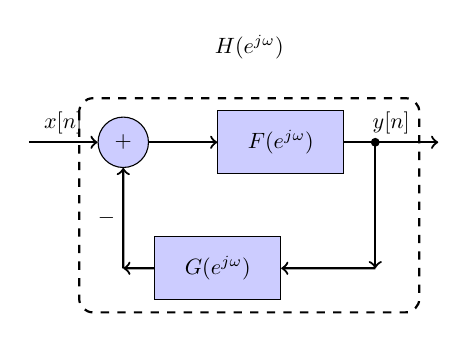
\begin{tikzpicture}[scale=0.8, every node/.style={scale=0.8}]
        % Define styles
        \tikzset{
            block/.style={draw, rectangle, minimum height=1cm, minimum width=2cm, fill=blue!20},
            sum/.style={draw, circle, minimum size=8mm, fill=blue!20},
            arrow/.style={->, thick},
            system/.style={draw, dashed, thick, rounded corners=5pt}
        }
        
        % Place nodes
        \node[coordinate] (input) at (0,0) {};
        \node[sum] (sum1) at (1.5,0) {$+$};
        \node[block] (F) at (4,0) {$F(e^{j\omega})$};
        \node[coordinate] (output) at (6.5,0) {};
        \node[coordinate] (branch) at (5.5,0) {};
        \node[coordinate] (corner1) at (5.5,-2) {};
        \node[block] (G) at (3,-2) {$G(e^{j\omega})$};
        \node[coordinate] (corner2) at (1.5,-2) {};
        
        % Draw the system boundary (dotted box around F, G, and sum)
        \draw[system] (0.8,0.7) rectangle (6.2,-2.7);
        
        % Draw arrows
        \draw[arrow] (input) -- node[above] {$x[n]$} (sum1);
        \draw[arrow] (sum1) -- (F);
        \draw[arrow] (F) -- node[above] {$y[n]$} (output);
        \draw[arrow] (branch) -- (corner1);
        \draw[arrow] (corner1) -- (G);
        \draw[arrow] (G) -- (corner2);
        \draw[arrow] (corner2) -- node[left] {$-$} (sum1);
        
        % Label overall system - moved outside the box
        \node[above] at (3.5,1.2) {$H(e^{j\omega})$};
        
        % Mark branch point
        \fill (branch) circle (2pt);
    \end{tikzpicture}
    \end{center}
    
    \vspace{5cm}

    % \newpage
    
    \item \textbf{(6 points)} Find $G(e^{j\omega})$ such that $H(e^{j\omega}) = 1$. Is the system $G(e^{j\omega})$ stable?
    
    \textbf{Note:} By achieving $H(e^{j\omega}) = 1$, we're effectively controlling the system $F(e^{j\omega})$. That is, we're making $F(e^{j\omega})$ produce whatever output we set it.
    
    \vspace{4cm}
\end{enumerate}

\ifthenelse{\boolean{showresults}}{
\vspace{0.5cm}
\textbf{Solutions:}

\begin{enumerate}[label=(\alph*)]
    \item \textbf{Finding the frequency response $F(e^{j\omega})$:}
    
    Taking the DTFT of both sides:
    \[
    Y(e^{j\omega}) + 4e^{-j2\omega}Y(e^{j\omega}) = X(e^{j\omega}) - 0.5e^{-j\omega}X(e^{j\omega})
    \]
    
    Therefore:
    \[
    \boxed{F(e^{j\omega}) = \frac{1 - 0.5e^{-j\omega}}{1 + 4e^{-j2\omega}}}
    \]
    
    \textbf{Causal:} Yes, \textbf{Stable:} Yes
    
    \item \textbf{Overall system:}
    \[
    \boxed{H(e^{j\omega}) = \frac{F(e^{j\omega})}{1 + F(e^{j\omega})G(e^{j\omega})}}
    \]
    
    \item \textbf{Finding $G(e^{j\omega})$:}
    \[
    \boxed{G(e^{j\omega}) = \frac{-0.5e^{-j\omega} - 4e^{-j2\omega}}{1 - 0.5e^{-j\omega}}}
    \]
    
    \textbf{Unstable} due to pole outside unit circle.
\end{enumerate}
}{}







\end{enumerate}



% -------------------------------------------- Equations PAGE --------------------------------------------
\newpage

\begin{center}
\textbf{Reference Formulas}
\end{center}

\vspace{0.5cm}

% \section*{Basic Functions and Identities}

\textbf{Euler's Identity:}

\[
e^{j\omega} = \cos(\omega) + j\sin(\omega)
\]

\textbf{Unit Step Function:}
\[
u[n] = \begin{cases}
1 & \text{if } n \geq 0\\
0 & \text{if } n < 0
\end{cases}
\]

\textbf{Unit Impulse Function:}

\[
\delta[n] = \begin{cases}
1 & \text{if } n = 0\\
0 & \text{if } n \neq 0
\end{cases}
\]

\textbf{Impulse Sampling Property:}
\[
x[n]\delta[n-k] = x[k]\delta[n-k]
\]

% \section*{Discrete-Time Fourier Transform}

\textbf{DTFT (Analysis):}

\[
X(e^{j\omega}) = \sum_{n=-\infty}^{\infty} x[n]e^{-j\omega n}
\]

\textbf{Inverse DTFT (Synthesis):}
\[
x[n] = \frac{1}{2\pi}\int_{-\pi}^{\pi} X(e^{j\omega})e^{j\omega n}d\omega
\]

% \section*{Convolution}

\textbf{Convolution Sum:}

\[
y[n] = x[n] * h[n] = \sum_{k=-\infty}^{\infty} x[k]h[n-k] = \sum_{k=-\infty}^{\infty} h[k]x[n-k]
\]

\textbf{Convolution Property:}
\[
x[n] * h[n] \overset{\text{DTFT}}{\longleftrightarrow} X(e^{j\omega})H(e^{j\omega})
\]


% \section*{Useful Identities}

\textbf{Geometric Series:}

\[
\sum_{n=0}^{\infty} ar^n = \frac{a}{1-r} \quad \text{for } |r| < 1
\]

\[
\sum_{n=0}^{N-1} ar^n = a\frac{1-r^N}{1-r} \quad \text{for } r \neq 1
\]

\textbf{Trigonometric Identities:}
\[
\cos(\omega) = \frac{e^{j\omega} + e^{-j\omega}}{2}, \quad \sin(\omega) = \frac{e^{j\omega} - e^{-j\omega}}{2j}
\]

\newpage
\begin{center}
\textbf{DTFT Tables}
\end{center}

% \subsection*{Table 1: Symmetry Properties of the DTFT}
\begin{center}
\includegraphics[width=0.55\textwidth]{Figures/table2p1.png}
\end{center}

% \subsection*{Table 2: DTFT Transform Theorems}
\begin{center}
\includegraphics[width=0.55\textwidth]{Figures/table2p2.png}
\end{center}

% \subsection*{Table 3: Fourier Transform Pairs}
\begin{center}
\includegraphics[width=0.55\textwidth]{Figures/table2p3.png}
\end{center}






\end{document}